%%%%%%%%%%%%%%%%%%%%%%%%%%%%%%%%%%%%%%%%%%%%%%%%%%%%%%%%%%%%%%%%%%%%%%%%%%
% Copyright (c) 2011, ETH Zurich.
% All rights reserved.
%
% This file is distributed under the terms in the attached LICENSE file.
% If you do not find this file, copies can be found by writing to:
% ETH Zurich D-INFK, Haldeneggsteig 4, CH-8092 Zurich. Attn: Systems Group.
%%%%%%%%%%%%%%%%%%%%%%%%%%%%%%%%%%%%%%%%%%%%%%%%%%%%%%%%%%%%%%%%%%%%%%%%%%

\documentclass[a4paper,twoside]{report} % for a report (default)

\usepackage{bftn,color} % You need this
\usepackage{verbatim} % for comment

\title{Routing in Barrelfish}   % title of report
\author{Akhilesh Singhania}	% author
\tnnumber{006}  % give the number of the tech report
\tnkey{Routing} % Short title, will appear in footer

% \date{Month Year} % Not needed - will be taken from version history

%% \newcommand{\note}[1]{}
\newcommand{\note}[1]{[\textcolor{red}{\textit{#1}}]}

\begin{document}
\maketitle

%
% Include version history first
%
\begin{versionhistory}
\vhEntry{1.0}{09.06.2010}{AS}{Initial version}
\vhEntry{1.01}{14.06.2010}{AS}{Added discussion of design and unresolved issues}
\vhEntry{1.02}{23.07.2010}{AS}{More work on design and API}
\end{versionhistory}

% \intro{Abstract}		% Insert abstract here
% \intro{Acknowledgements}	% Uncomment (if needed) for acknowledgements
% \tableofcontents		% Uncomment (if needed) for final draft
% \listoffigures		% Uncomment (if needed) for final draft
% \listoftables			% Uncomment (if needed) for final draft

\chapter{Motivation}

We motivate the reasons to use a routing layer and group communication in Barrelfish.

\section{Fully connected assumption}
Most current multicore machines are fully connected via shared memory.
Any core in the system can communicate with any other core in the system
by using shared memory.
Most applications are also designed accordingly.

However, this assumption may not hold in the near future.
On SCC, the set of memory a core can access is determined by the setup of its
Look Up Tables (LUTs).
It is possible that these tables are setup in such a manner that
two or more cores do not have access to the same region of memory.
In such cases to communication these cores will have to route
via another set of cores if such a path exists.

If we operate Barrelfish on a cluster of machines,
only the core(s) where the network stack is running
has the ability to communicate with other machines.
Other cores in the system have to route their messages through this core(s).

These are some examples of current setups which are not fully connected.
Based on this, we anticipate that the fully connected assumption
on future machines may not hold.

A routing layer akin to the one in IP routing will allow applications to communicate in
such environments without the application having to worry about
how the message gets there.
The application can specify the core or set of cores it wishes the message be sent to
and the routing library will properly route it.

\section{Heterogeneous IDC}
Barrelfish supports various IDC mechanisms.
Different mechanisms provide different semantics and guarantees such as maximum frame
size, notification mechanism, synchrony, etc.

An application can utilize multiple IDC mechanisms.
This can happen if a homogeneous machine supports multiple IDC mechanisms or if the
application runs on a heterogeneous machine.
To avoid the need for the application to understand the different semantics of all IDC,
it can conform to the semantics provided by the routing library.

The semantics provided by the routing layer are discussed in section \ref{sec:semantics}.

\section{Group communication}

Various parallel computing abstractions such as barriers
require communication among a group of threads.
When any thread enters a barrier, it waits for all other threads to enter
the barrier as well before continuing.

Various distributed communication abstractions such as achieving consensus
also require communication among a group of nodes.
A group of nodes that want to come to agreement on some value
need to communicate with each other.

\cite{nishtala:optimizing-collective:hotpar09, barrelfish:sosp09}
showed that even in a fully connected 
machine, using some form of routing can improve the performance of group communication.
The sender sends the message to a subset of nodes it wishes to communicate with.
The subset will in turn forward it to the remaining set of nodes.
The work has also shown that the order in which messages are sent also matters.
The optimal route and ordering of messages is machine dependent.

If applications were written with the abstraction of a group layer,
it will allow the library sufficient flexibility in
selecting the optimal route based on the machine type.

\section{Resource cost}
Communication channels cost resources.
The more channels that exist, the more resources will be utilized.
The resources we discuss are memory, cache, and CPU.

\subsection{Memory}
A channel of any type will require some memory to buffer unsent messages and
messages that have been received but not delivered.
The UMP channel using x86 machines requires additional memory for the channel itself.
The amount of memory required is governed by the number of messages in flight and
the number of messages in buffer.

\subsection{CPU}
The UMP channel implementation on x86 requires explicit polling
to check for new incoming messages.
The more channel a core has, the more time will be spent polling.

\subsection{Cache}
The UMP channel implementation on x86 has to poll the channel to check
if there is a pending message on the channel.
The polled cache line if it is not in the cache is pulled in.
If the core has many channels, much of its cache will be flushed
due to polling the channels.

\subsection{Summary}
The more channels a core has, the more memory is required to construct them,
the more CPU time is required to poll them, and the more cache is flushed to poll them.
These are all detrimental to a well performant system.

By limiting the number of channels, we will limit the amount of resources required.
One way to limit the number of channels is to not construct a fully connected network
where all cores have a channel to each other.
Instead some cores can forward messages on behalf of other cores in the system.

\chapter{Design}

\section{Terminology}

\textbf{Node:}
A node is an instance of the routing library on a dispatcher.

\textbf{Groups:}
The set of all nodes on the machine form a \emph{universe group}.
The set of nodes in the universe group that
wish to communicate with each other form an \emph{application group}.
An application group is a subset of the universe group.
A subset of nodes in the application group can form a \emph{multicast group}.

It is possible to join and leave any multicast and application group.

\textbf{IDs:}
Each application group is identified by a \emph{group ID}.
The group ID in turn identifies the instance of routing library to use.
The group ID is unique within the universe group.

Each multicast group is identified by \emph{multicast ID}.
The multicast ID is unique within the application group.

When nodes join an application group, they are assigned a \emph{node ID}.
The node ID is unique within the application group.

Each node is also given an \emph{application broadcast ID}.
These may or may not be unique and are drawn from a set that
may just have a single element.

The union of the set of node ID, multicast ID, and application broadcast ID is
called the \emph{destination ID}.
The set of node IDs, multicast IDs, and application broadcast IDs are disjoint.

\textbf{Messaging:}
It is not possible to communicate with nodes in the universe group that
are not in the application group.

A node can send a message to another node in the application group by
sending a message to the appropriate node ID.
A node can send a message to all nodes in the application group by
sending a message to the application broadcast provided to it.
A node can send a message to all nodes in an multicast group by
sending a message to the multicast ID provided to it
when it joined the multicast group.

\textbf{Types of messages:}
\emph{Unicast:} Send a message to a single node in the application group.
\emph{Broadcast:} Send a message to all nodes in the application group.
\emph{Multicast:} Send a message to all nodes in the multicast group.

\textbf{Forwarding table:}
Forwarding tables enable messaging.
Each node has an associated forwarding table.
The table is a list of tuples called \emph{table entries}.
The first item in the tuple is an element from the set of destination IDs.
The second item in the tuple is a list of node IDs
also called the \emph{destination set}.

When a message is received from either the application layer or
from another node, it is sent onwards to the nodes in the destination set.
If the node itself is specified in the destination set,
then the message is delivered to the application layer.

The forwarding table is setup to enable the three types
of messaging discussed above.
Any node in the application group can message
any other node in the application group.
Any node can send a broadcast message to all nodes in the application group.
Any node can send a message to any multicast group if any exist.
Note that the node need not be part of the multicast group
to send a message to it.

We may support link state style or distance vector style routing.
In link state the nodes have complete knowledge of all links in the group
and know how to reach all other nodes in the group.
In distance vector style, the nodes may not have all information in the group,
in this case, they will have a default node that the message is forwarded to
which may or may not have the appropriate information.
Like IP routing, their can be multiple default nodes
for different range of nodes.

\section{Semantics}\label{sec:semantics}

The routing layer will provide a uniform set of semantics to the
application layer regardless of the set of semantics the
IDC mechanisms below it provide.
It can provide different semantics to suit the
needs of different application scenarios.

Below, we discuss the different set of semantics it can provide.

\subsection{Set 1: Single source FIFO}
The set of semantics provided are as follows:

\begin{itemize}
\item Reliability:
  A message is delivered only once and only if it was sent earlier.
  Each message is eventually delivered and the contents are not corrupted.
\item Single source FIFO ordering:
  If a sender sends $m$ before $m'$ then $m$ is delivered before $m'$
  at all receivers.
\item Failure:
  The routing library will not fail.
\item Payload:
  The IDC can deliver an arbitrarily sized message.
\end{itemize}

\subsection{Set 2: Causal order}
The set of semantics provided are as follows:

\begin{itemize}
\item Reliability:
  A message is delivered only once and only if it was sent earlier.
  Each message is eventually delivered and the contents are not corrupted.
\item Causal ordering:
  If the delivery of message $m$ depends upon the delivery of message $m'$ as
  per the \emph{happened before} relationship \cite{events-time},
  then $m$ is not delivered till $m'$ has been delivered.
\item Failure:
  The routing library will not fail.
\item Payload:
  The IDC can deliver an arbitrarily sized message.
\end{itemize}

\subsection{Set 3: Total order}
The set of semantics provided are as follows:

\begin{itemize}
\item Reliability:
  A message is delivered only once and only if it was sent earlier.
  Each message is eventually delivered and the contents are not corrupted.
\item Total order:
  All messages are delivered to all nodes in the same order.
\item Failure:
  The routing library will not fail.
\item Payload:
  The IDC can deliver an arbitrarily sized message.
\end{itemize}

It is possible to order messages using various types of ordering mechanisms.
Investigation of this remains future work.

\subsection{Additional sets}
In future, if we choose to provide additional set of semantics,
they will be listed here.
They could include weaker semantics than above if the underlying IDC mechanism
are too expensive.
Some example are just reliability, or not even providing reliability.

\section{Interface}
We discuss the interface for group management and sending/receiving of messages.

\subsection{Group management}

\textbf{Creating groups:}
Before nodes can join a group, they need to be created.
Any dispatcher in the system can create a new application group
and any node in an application group can create a new multicast group
within the application group.

The library will return to application a group ID or
multicast ID of the created group.

\textbf{Updating a group:}
A dispatcher can join any application group by calling join on
the application group ID.
A node can join any multicast group within the application group it is part of.
When the join has finished, the node gets the join callback from the library.
When a dispatcher is done joining an application group,
it can query the library for its node ID and application broadcast ID.

Similarly a node can leave a group at anytime by calling leave on the group ID.
When the leave is done, the application will get a leave callback.
A dispatcher should call leave before it exits the system.

The behavior of the group is undefined while membership is in flux.
New links are being created and old links are being torn down.
Messages may not reach their proper destination.
If such guarantees are required at all times in the application,
the application must refrain from sending messages while
group member is in flux.

\section{Flow control}
The IDC mechanisms that the routing library operates over are asynchronous.
When a message is sent over them,
it will eventually be delivered to the receiver.
Undelivered messages are maintained in a queue of fixed length.
If the sender tries to send messages too quickly the queue can fill up.
If the queue is full, the sender must wait
till the queue has room for more messages.
IDC mechanisms allow senders to register callbacks in such situations.
When a send fails with the transient error that
the queue is full, the sender can register
a callback which will be called when the next send should not fail.
While the sender waits for the callback, it has to handle the unsent message.

We discuss the simple scenario of two nodes and
then a more complex scenario of many nodes.

\subsection{Client-server model}

\begin{figure}[t]
 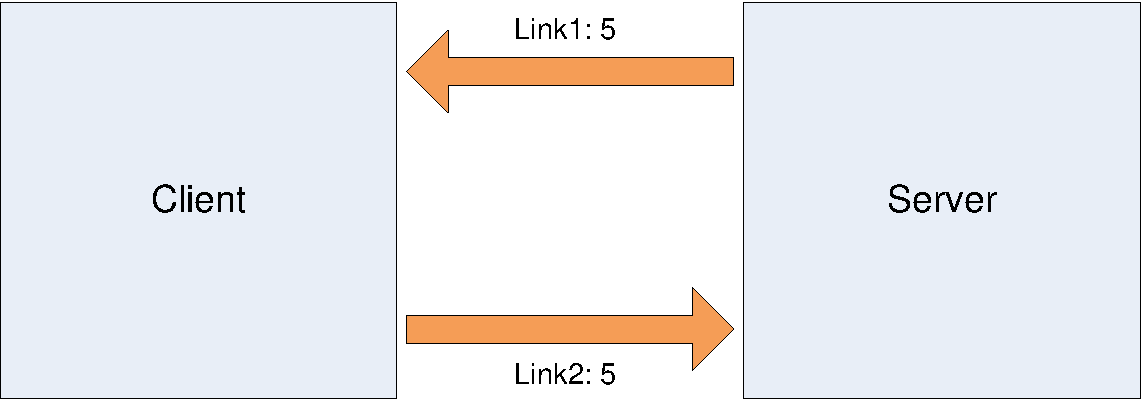
\includegraphics[width=\columnwidth]{client-server.pdf}
 \caption{Client-server model}\label{fig:client-server}
\end{figure}

Figure \ref{fig:client-server} shows a simple client-server model
of two nodes that are directly connected.
The weights on the edges is the length of the queue.
The client sends messages to the server, the server processes them
and sends replies to the client.
It is possible that link1 becomes full maybe because
the client has not been handling replies on it.
At this point the server has some options:

\begin{itemize}
\item Drop the message.
  The server can simply drop the message if the queue is full.
  This will result in an unreliable channel.
\item Allocate some resources and queue the message up.
  This implies unbounded resource requirement.
\item Apply back pressure on the client.
  The server at this point can stop processing messages
  from the client till it is able to send messages to it again.
\end{itemize}

In this model the last option works well as it will force the client
to slow down and process replies before sending more requests.

\subsection{Multihop route}

\begin{figure}[t]
 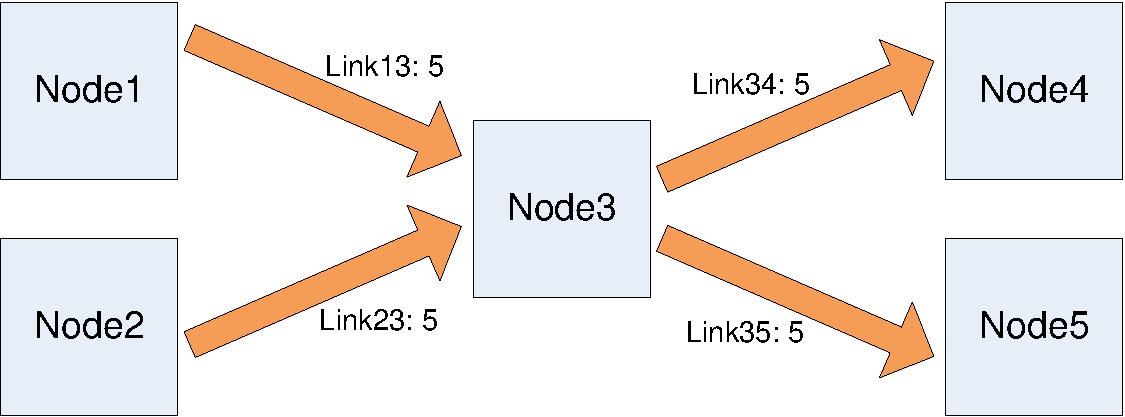
\includegraphics[width=\columnwidth]{many-to-many.pdf}
 \caption{Example multihop route}\label{fig:many-to-many}
\end{figure}

In this scenario the problem is more complex.
Figure \ref{fig:many-to-many} shows a group of 5 nodes,
the link weights specifies the queue length of the link.
If node1 and node2 are sending messages to node4,
link34 will fill up before link13 or link23 does.
Node3 cannot send additional messages to node4.
At this point, node3 has the following options:

\begin{itemize}
\item Continue to process incoming messages on link13 and link23.
  If they are destined for node4, drop them.
  This will result in an unreliable channel.
\item Continue to process incoming messages and if they are destined for node4,
  queue them up locally.
  This implies unbounded resource requirement.
\item Stop processing messages on link13 and link23.
  This will delay messages on those links that were not destined to node4.
  In literature, this is called \emph{Head of line blocking} \cite{cite}.
\end{itemize}

None of these solutions are particularly desirable.
Flow control in the context different types of networks has
been studied previously.
We should study the related work before we come up with our own designs.

I summarize some existing work I am aware of here that we should look into:
\begin{itemize}
\item Credit based flow control:
  The endpoints dictate maximum number of messages in flight.
\item TCP flow control
\item Ethernet flow control
\item Datacenter ethernet flow control
\item Related work in routing between sockets on a machine
\item QoS (DiffServ and IntServ).
\end{itemize}

Some applications may not be willing to pay the cost of flow control.
Further, a flow control mechanism that guarantees reliability
may not scale well with  number of nodes.
This can be an interesting research topic for us.

We discuss some abstract ideas we have for flow control below.

\subsubsection{Reservation of resources with end-to-end flow control}
The essential idea is that when a route is established,
reservations for some number of in flight messages are made for the route.
Even though the links might be shared,
no other routing path is allowed to use the reserved resources.
The endpoints must then limit the number of in flight messages.
If they exceed it, the library can deliver an error at the endpoint or try to
optimistically deliver the message and drop the message if it is unable to.

For example, in figure \ref{fig:many-to-many},
if reservations for two messages is made for the routing path
from node1 to node4, node1 and node3 each will maintain a queue of size 2.
Whenever they receive a message from the application in node1 destined to node4
and they are not able to send it on the link,
they can locally store the message.
Eventually, when the link has space in it,
they can try to send the message again.

It remains to be seen if the approach can work and scale well.
\note{Cite work on switching networks and other works that make reservations and
  give guarantees.}

This approach works when the nodes that are sharing the links
cooperate with one another.
However, if the link is shared between distrustful
nodes then additional guarantees of fairness and no starvation maybe required.

\begin{figure}[t]
 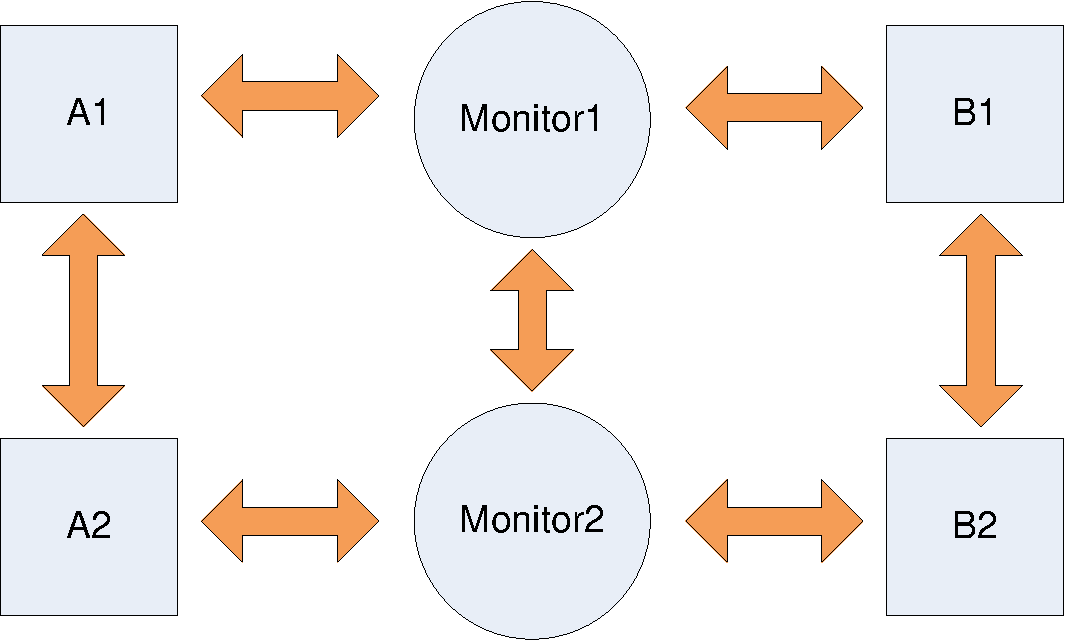
\includegraphics[width=\columnwidth]{client-monitor.pdf}
 \caption{A network of monitor with clients}\label{fig:client-monitor}
\end{figure}

Figure \ref{fig:client-monitor} shows a network of two monitors.
Each monitor is connected to two clients.
Clients A1 and A2 are cooperating and client B1 and B2 are cooperating.
The clients want to send some messages that must go through the monitors such as
transferring capabilities.
If one pair of client is aggressive in sending messages,
it may fill up the link between the monitors and impact the performance
of the other pair of clients.
In this scenario, the link between the monitor can be seen
as a common system resource that is being multiplexed between the users.
The monitors should guarantee some fairness to the users in using this link.

\section{Open questions}
Some open questions

\subsection{Discovering node IDs}
When a set of dispatchers join an application group,
each of them is assigned a node ID.
The nodes need some mechanism of discovering the IDs of each other
so that they can message each other.

The discovery service will be built on top of the routing library
and can be designed in multiple ways.
Nodes can send broadcasts to each other informing each other of their node IDs,
they can use the name service, etc.

\chapter{Interesting benchmarks}\label{chap:benchmarks}

Some benchmarks that validate the claims of above and show the performance of the library.

\note{Costs of one-to-many channels. One sender, multiple readers.}

\note{Comparison of routes with no forwarding and routes with forwarding.}

\note{Resource requirements for channels, memory and cpu time.}

\note{Cost of the discussion group membership update mechanism.}

\chapter{Fun research questions}

\begin{itemize}
\item Flow control
\item Link state vs. distance vector routing
\end{itemize}

\bibliographystyle{abbrvnat}
\bibliography{defs,barrelfish}

\end{document}
